\documentclass{crypto-exercise}
\usepackage{amsthm}
\usepackage{float}
\author{Sven Laur}
\contributor[Initial solution]{Sanja Scepanovic}
\contributor[Changed notation and added material]{Sven Laur}
\editor{Sven Laur}
\tags{hypothesis testing, false positives, false negatives, tradeoff}

\newcommand{\CTOSS}{\mathsf{CoinToss}}

\begin{document}
\begin{exercise}{Tradeoffs between false positives and false negatives}
Let $\AD$ be a $t$-time distinguisher and let $\alpha(\AD) = \pr{\AD(x) = 0|\HHH_1}$ be the ratios of false negatives and
$\beta(\AD) = \pr{\AD(x) = 1 | \HHH_0}$ be  the ratio of false positives.
Show that for any $c$ there exists a $t + O(1)$-time adversary $\ADB$ such that
$$\alpha(\ADB) = c \cdot \alpha(\AD) \quad \text{and} \quad \beta(\ADB) = (1-c) + c \cdot \beta(\AD).$$
Give some real world examples where such trade-offs are economically justified.
\end{exercise}
\begin{solution}
Let $\CTOSS(c)$ denote the binary distribution created by tossing a $c$-biased coin, i.e.,
\begin{align*}
 \pr{b\gets\CTOSS(c):b=0}=1-c
 \qquad\text{and}\qquad 
 \pr{b\gets\CTOSS(c):b=1}=c\enspace.
\end{align*}
It is relatively easy to implement such a procedure given access to a fair coin. For instance, we can create $\frac{3}{8}$-biased coin by first making three fair coin tosses and outputting one if the outcome is either $000$, $001$ or $010$. In general, we need $n-1$ tosses of a fair coin to approximate the output of a biased coin with an error $2^{-n}$. Moreover, the procedure is really efficient, as the decision procedure corresponds to a single comparison. 


Armed with this knowledge, we can define a new distinguisher $\ADB$ that uses $\AD$ as a subroutine:
\begin{align*}
\begin{fblock}{\ADB(x)}
& b\gets\CTOSS(c)\\
& \IF c=1\ \THEN \RETURN \AD(x)\\
& \ELSE \RETURN 1
\end{fblock}
\end{align*}
For fixed bias $c$, the overhead in the running time of $\ADB$ is constant. However, it is also interesting to consider $c$ as a varying parameter. Let $n$ be the number of fair coin-tosses inside $\CTOSS$ procedure. Then we can coose the parameter $c$ from the set $\set{\frac{0}{2^n},\frac{1}{2^n},\ldots, \frac{2^n}{2^n}}$ without changing the computational complexity.  

By the construction it is straightforward to express: 
\begin{align*}
\pr{\ADB(x) = 0|\HHH_1} &= \pr{b\gets\CTOSS(c):b=1} \cdot \pr{ \AD(x) = 0 | \HHH_1} \\
\pr{\ADB(x) = 1|\HHH_0} & =\pr{b\gets\CTOSS(c):b=0 } +  \pr{b\gets\CTOSS(c):b=1} \cdot \pr{ \AD(x) = 1 | \HHH_0 }\enspace
\end{align*}
and thus the ratio of false negatives and false positives for  new algorithm are
\begin{align*}
\alpha(\ADB)&=\pr{\ADB(x) = 0|\HHH_1} = c \cdot \alpha (\AD)\\
\beta(\ADB)&=\pr{\ADB(x) = 1|\HHH_0}= (1-c) + c \cdot \beta(\AD)\enspace.
\end{align*}
Figure~\ref{fig:tradeoffs} shows how the choice of $c$ influences these ratios. The blue line shows the tradeoffs achievable with the construction given above. The read line shows the tradeoffs achievable by the symmetric construction.

\begin{figure}[H]
\begin{center}
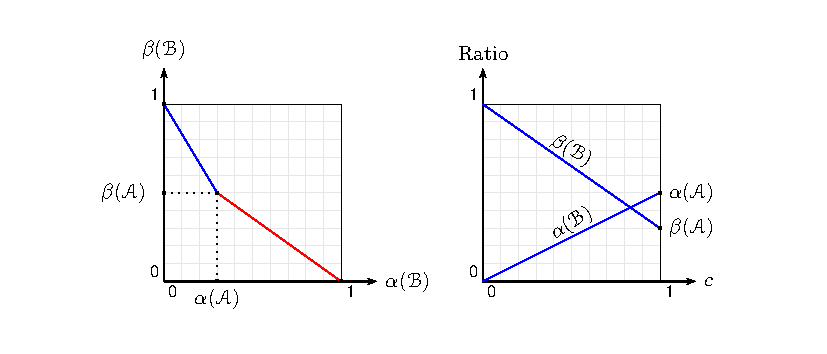
\includegraphics{figures/0303-tradeoffs}
\end{center}
\caption{Various achievable tradeoffs between false positives and false negatives}
\label{fig:tradeoffs}
\end{figure} 

\noindent 
Note that the tradeoff is not without cost. Recall that we can always keep the aggregate error $\gamma(\AD)\leq 1$ by inverting the output if necessary. Hence, the aggregate error 
\begin{align*}
 \gamma(\ADB)=(1-c)+c\gamma(\AD)= \gamma(\AD) + (1-c)\cdot(1-\gamma(\AD))
\end{align*}
always increases as long as $c$ decreases.  The effect is larger for good distinguishers that have smaller the aggregate error. 
 
\vspace*{2ex}
\noindent
\textsc{Practical applications.} 
In practice, the cost of making false positive and making false negative errors is not the same. For instance, if a bank gives out  loans, then the false positives are companies or persons who should not get the loan because they cannot afford it. In this case, making a false positive decision can cost millions dollars, while not giving a loan as much smaller penalty. In healthcare, the situation can be reversed. Usually, a false positive diagnosis is not a problem, as further studies correct the diagnosis while undetected cancer can cause severe complications or even death.    

\end{solution}
\end{document}